\cleardoublepage
\chapter{Implementation}
\label{ch:implementation}

\section{Implementing the Multiparty SJ Compiler}

\subsection{Revised Parser Generator}
\label{subsec:ppgimpl}

As discussed in \autoref{subsec:extendingparsegen} the parser generator needs to be extended to handle the additional syntax of MPSJ. The code fragment in \autoref{LSTparsegen} shows how the type declaration is extended. 

The declaration of the global protocol is defined as a type declaration in lines 1-3. Lines 5-9 define the structure of the global protocol as a set of optional modifiers such as \LST{private} or \LST{public}, the \LST{global_protocol} keyword and an identifier, which can be any expression normally used for variable names. The rest of the definition is the global session type itself enclose in braces. 

The main purpose of the parser is to parse the syntax and build the Abstract Syntax Tree. The tree is built from AST Nodes, which get created through the node factory. The call to the node factory is made in line 8 and the information from each of the syntactic elements is passed into the method in form of arguments.  

\begin{lstlisting}[basicstyle=\LISTINGSTYLE, numbers=left, caption={Example code fragment showing the language extension to the parser generator}, label={LSTparsegen}]
extend type_declaration ::=
	sj_glob_protocol_declaration:a
	{: RESULT = a; :};

sj_glob_protocol_declaration ::=
	modifiers_opt:a SJ_GLOB_PROTOCOL IDENTIFIER:n LBRACE sj_glob_session_type_body:t RBRACE:r
	{: 
		RESULT = parser.nf.SJGlobProtocolDecl(parser.pos(a, r), a, parser.nf.Id(parser.pos(n), n.getIdentifier()), t); 
	:};

sj_glob_session_type_body ::= 
	sj_glob_session_type_element:a
	{: RESULT = a; :}
|	sj_glob_session_type_element:a DOT sj_glob_session_type_body:b
	{: RESULT = a.child(b); :};

sj_glob_session_type_element ::=
	sj_glob_session_type_element_prefix:a sj_communication_type_elem:b
	{: 
		RESULT = parser.nf.SJGlobTypeNode(parser.pos(a,b), a, b); 
	:};	
\end{lstlisting}

Other syntactic elements are implemented in a similar fashion. A global session type body can consist of one element or multiple elements in form of \textit{children}. The language-independent syntax definition supports recursivity, such as in line 14, which can decompose a sequence of session type elements into elements and their children.

One of the points of integration with the current SJ Compiler is depicted in line 18, showing a global type element as conjunction of a prefix and an SJ communication type element. The latter, is an SJ operation such as a send or receive already used in SJ. The definition of such constructs as non-terminal tokens allows extension to the implementation to be integrated smoothly.  


\subsection{Inferring the List of Participants}
\label{subsec:inference}

The list of participants is a set of unique participants included in a global session type, which will then be translated into class members of the global protocol class. 

Each \LST{SJGlobElementPrefixNode} stores the parties for each global type element, such as a send operation, in form of \LST{Id} fields. The first element in the prefix is referred to as the \textit{principal}, as the operation type directly refers to that party, whereas the latter party is referred to as its \textit{partner}.

Two types of list are required for the inference of all participants in a global session type. 

\begin{lstlisting}[basicstyle=\LISTINGSTYLE]
	LinkedList<Id> participants = new LinkedList<Id>();
	LinkedList<String> names = new LinkedList<String>();
\end{lstlisting}

The list of \LST{Id}s stores the unique set of participants, whereas the list of \LST{String}s holds their names. This is necessary due to the fact that the same participants at different points in the global type will have different \LST{Id} nodes. They can therefore only be compared in terms of their names.

The participant inference algorithm adds both participants in the prefix of the first element to both lists by default, as actions as reflexive operations are not permitted, i.e. the two participants will always be distinct. 

\begin{lstlisting}[basicstyle=\LISTINGSTYLE, numbers=left]
while(child != null) {
			
	if(!(names.contains(child.getPrefix().getPrincipal().toString())))
	{
		participants.add(child.getPrefix().getPrincipal());
		names.add(child.getPrefix().getPrincipal().toString());
	}
	if(!(names.contains((child.getPrefix().getPartner().toString())))) 
	{
		participants.add(child.getPrefix().getPartner());
		names.add(child.getPrefix().getPartner().toString());
	}
	
	child = child.child();	
}
\end{lstlisting}

The algorithm then proceeds recursively through all the global type elements' children and compares each participant in each prefix against the \LST{String} list. If the name is not included in the list, the participant's \LST{Id} is added to the list.


\subsection{Generating the Global Protocol Class}

The global protocol class is built purely from the global session type. The \LST{SJGlobProtocolDecl} node extends the \LST{polyglot.ast.ClassDecl} node and passes the necessary arguments into the \LST{super} constructor.

The \LST{Id} and \LST{Flags} are transferred in directly and the superclass is set via a \textit{canonical type node} to the runtime class \LST{SJGlobSession}. \LST{SJGlobSession} provides the methods for inviting participants and accepting invitations.

The superclass constructor also takes in a \LST{ClassBody} parameter. This is the challenging element of the global protocol class creation, where the session participants are added. The class body members are created by the static method \LST{makeGlobProtocolMembers} which in turn calls the \LST{createParticipantList} method discussed in \autoref{subsec:inference}. All members are made \LST{public} by the compiler in order to be accessible by the MPSJ code from outside the protocol. The newly created body is then fed into the \LST{ClassDecl} constructor. 

The \LST{SJGlobParticipant} fields are then initialised during the \LST{SJProtocolDeclTranslator} compiler pass. Throughout the entire compilation process all nodes are immutable. Any changes to a node are performed on its copy and the modified copy is then returned to replace the original.

\begin{lstlisting}[basicstyle=\LISTINGSTYLE, numbers=left]
	private Node translateSJGlobProtocolDecl(SJGlobProtocolDecl pd) throws SemanticException
	{		
		Position pos = pd.position();
		QQ qq = new QQ(sjts.extensionInfo(), pos);
		
		List<ClassMember> members = pd.body().members();
		List<ClassMember> newMembers = new LinkedList<ClassMember>();	
		
		for(ClassMember mb: members) {
			if(mb instanceof FieldDecl) {
				List<Object> mapping = new LinkedList<Object>();
				String translation = "new SJGlobParticipant(%E)";
				mapping.add(sjnf.StringLit(pos, ((FieldDecl) mb).name()));
			
				New n = (New) qq.parseExpr(translation, mapping);
				newMembers.add(((FieldDecl) mb).init(n));
			}
		}
		return pd.body(pd.body().members(newMembers));
	}
\end{lstlisting}

The method uses the QuasiQuoter library from \LST{polyglot.qq} which allows parsing Strings into AST nodes. This technique involves replacing the expression placeholder \LST{\%E} in line 12 by the name of the participant and parsing the complete expression into a \LST{New} node in line 15. The \LST{New} node corresponds to a \LST{SJGlobParticipant} constructor call, which takes in a \LST{String} argument to assign to the name of field of the participant class. The node is then addes as the initialiser field to the member via the method \LST{init} in line 16. The \LST{return} statement replaces the body of the original protocol by a new body with the modified members and returns the modified copy back to the compiler pass. The node is then replaced in the AST. 

\section{Implementing the Multiparty SJ Runtime}

\subsection{MPSJ Runtime Extension Structure}

The UML diagram in \autoref{fig:runtimeuml} effectively pictures the implementation details of \autoref{subsec:globprotocolcore}. Please note that this is a simplistic viewpoint of the actual implementation structure. Many methods, fields and dependencies are therefore omitted.

\begin{figure}[H]
\begin{center}
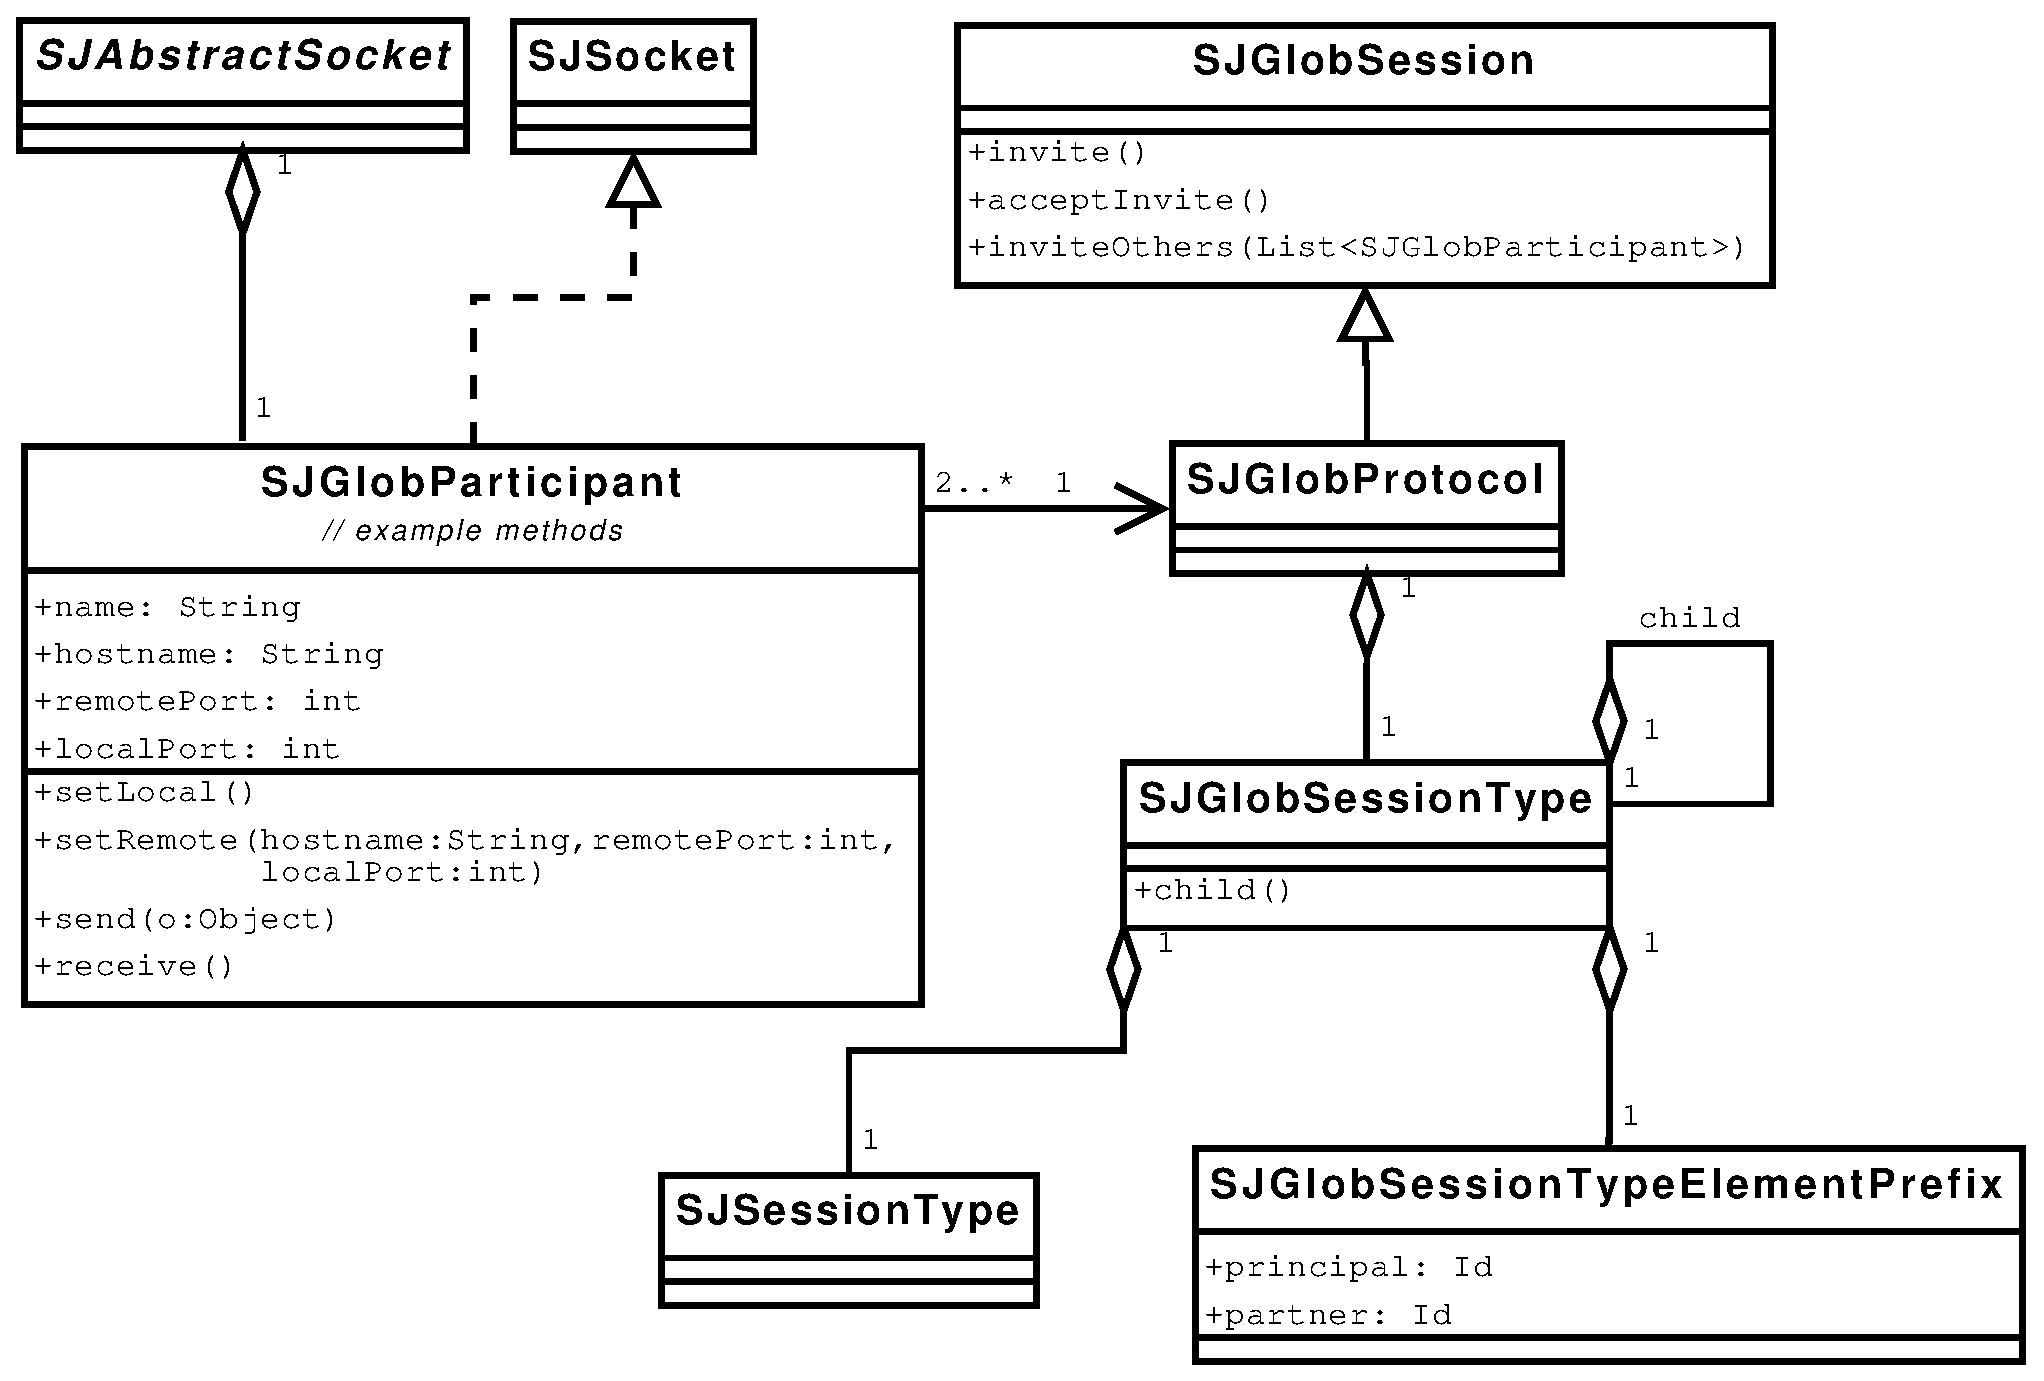
\includegraphics[width=0.875\textwidth]{uml}
\caption{UML diagram showing a fragment of the SJ Runtime Structure}
\label{fig:runtimeuml}
\end{center}
\end{figure}

The MPSJ Runtime reuses some of the compiler classes, such as the information about the session type of a session. As depicted, the \LST{SJGlobProtocol} class has a minimum number of two \LST{SJGlobParticipant} class members. These members implement the \LST{SJSocket} interface and delegate all their session operations to the \LST{SJAbstractSocket}. The information about the session is encoded in the \LST{SJGlobSessionType} and its child, the child of the child, etc. As discussed an \LST{SJGlobSessionType} consists of a standard \LST{SJSessionType} and an \LST{SJGlobSessionTypeElementPrefix} from which the participants of that operation can be obtained.


\subsection{Global Participants as Session Sockets}

The use of global participants as session sockets is one of the essential features of MPSJ which enhances the programming experience.

This achieved in the class \LST{SJGlobParticipant} which implements the \LST{SJSocket} interface. It would be possible to implement all the methods of this interface, however delegating the tasks to the \LST{SJAbstractSocket} member variable makes more efficient use of the exisiting code base.

Such an implementation also removes the need to specify seperate participant classes for accepting and initiating sockets as the \LST{SJAbstractSocket} behaves as an abstract superclass of all sockets. The socket is therefore inititated once the role of the participant is known, i.e. during session initiation.

Once the \LST{SJAbstractSocket} is initiated all operations such as sending and receiving are delegated from the global participant to the actual instance of the socket.

\subsection{Session Initiation and Acceptance Methods}

The invitation and acceptance methods are both implemented in the \LST{SJGlobSession} class from which all global protocol classes inherit. This enables the programmers to call these methods directly on the instances of their protocols and start or accept the session.

\paragraph*{The \LST{invite()} method} The procedure accesses the protocol and all its \LST{SJGlobParticipant} fields in order to set the sockets to the correct types and perform the connection initiation. The challenge is the lack of knowledge about the protocol class including the number of \LST{SJGlobParticipant} members, but the Java Reflection library\cite{javareflect} can be used to obtain this reflexive information about the structure of the class that calls the code. 

\begin{lstlisting}[basicstyle=\LISTINGSTYLE, numbers=left, caption=The session initiation method]
	public void invite() 
		{
		try {
			SJSessionParameters params = SJTransportUtils.createSJSessionParameters("d", "d");
			LinkedList<SJGlobParticipant> invitationList = new LinkedList<SJGlobParticipant>();
		
			for(Field f: getClass().getDeclaredFields()) {		
				if (f.getType().equals(SJGlobParticipant.class) && (!((SJGlobParticipant) f.get(this)).isLocal())) {		
					invitationList.add((SJGlobParticipant) f.get(this));			
				}
			}
			LinkedList<SJGlobParticipant> delegationList = new LinkedList<SJGlobParticipant>(invitationList);
		
			for(SJGlobParticipant gp: invitationList){			
				final SJService serv = SJService.create(null, gp.getHostname(), gp.getRemPort());
				gp.setDel(serv.request(params));
					
				delegationList.remove(gp);
				gp.send(delegationList);
			}
		} catch (Exception e) {e.printStackTrace();} 
	}
\end{lstlisting}

The code fragment from line 7 onwards iterates through all members of the class and checks if the member is of type \LST{SJGlobParticipant} and whether it has not been set to local by the programmer. When found, global participants are grouped into a list and a copy of the list is made for future reference.

For every remote participant in the list the \LST{invite()} method creates a connection with the participant's hostname and its port, both assigned earlier through the \LST{setRemote(..)} method. The method \LST{setDel(..)} in line 16 requests the connection with the remote participant and set the \LST{SJAbstractSocket} to the socket returned be the \LST{request(..)} method. This procedure is similar to the session establishment in SJ.

Following that the participant is removed from the copy of the list but all other participants remain on it. By sending the modified list (line 19) to the participant who just accepted the connection, we delegate further invitations of connections he has to establish to fullfil the circle. Note, that with every iteration through the original list, the \LST{delegationList} is shortened. Finally, when we reach the last element that list will be empty, as the last participant in the sequence does not have to establish connections with anyone. The initiating participant's role in the protocol from \autoref{fig:sessioncreation} is completed. 


\paragraph*{The \LST{acceptInvite()} method} This procedure is responsible for preparing all sockets for the acceptance of incoming connections. The main difference from the \LST{invite()} method is in lines 15-16. Additionally, no copy of the obtained participants' list is made or used.

\begin{lstlisting}[basicstyle=\LISTINGSTYLE]
	final SJServerSocket servsocket = SJServerSocketImpl.create(null, gp.getLocalPort(), params);
	gp.setDel(servsocket.accept());
	this.inviteOthers(gp.receive());	
\end{lstlisting}

For each participant in the session, the code fragment creates an accepting socket and sets the \LST{SJAbstractSocket} to the open socket returned by the \LST{accept()} method. All remote participants' sockets have to be set waiting for incoming connections on the agreed local ports, as it is unknown which session participant will initiate the session.

After establishing the connection the participant receives a list of all other participants who connections have to be established with. The establishment of these connections is taken care of in the \LST{inviteOthers(..)} method.

\paragraph*{The \LST{inviteOthers(..)} background method}

This method takes in an argument of type \LST{LinkedList<SJGlobParticipant>} and iterates through the list performing very similar actions to the \LST{invite()} method. The sockets on these participants, that have already been set to accepting sockets are now being overwritten to handle outgoing connections. Once the connection is established standards session operations may be performed via these channels.

Note that contrary to \LST{invite()} this method does not delegate any further invitations. The initialising party is the coordinator and therefore responsible for ensuring that all partners are linked to each other.